
\section{Results}

In the results section, the author describes his observations on the different models defined in section 3.4. The training used a batch size of 64. In total, each model was trained over 500.000 batches. \\

\begin{figure}[H]
    \centering
    \begin{subfigure}[b]{0.45\textwidth}
        \centering
        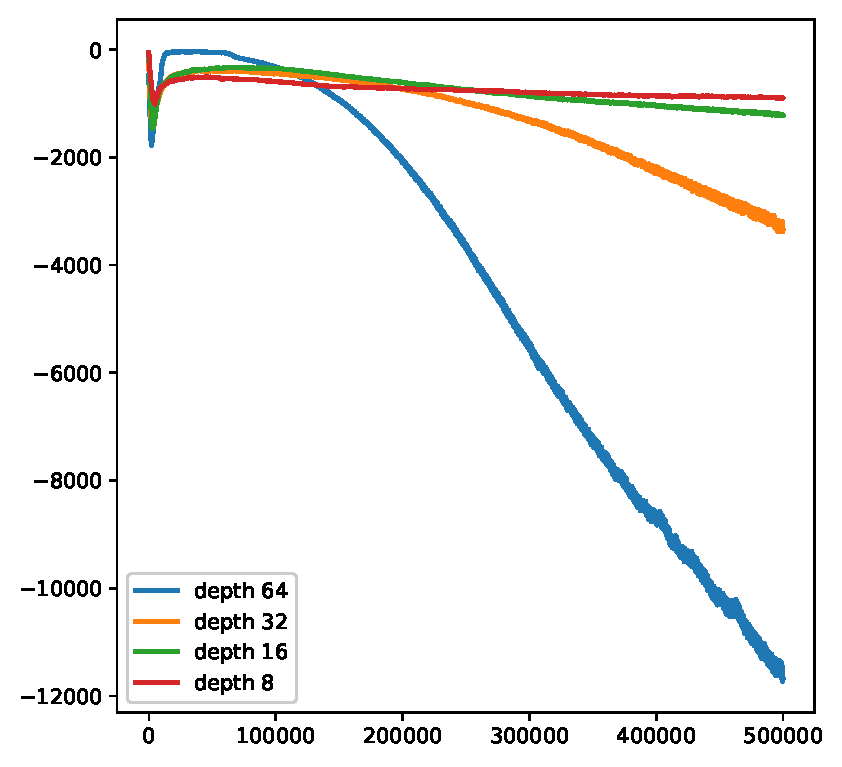
\includegraphics[width=\textwidth]{resources/images/celeba_hq_d_loss.eps}
        \caption{Anime Face}
        \label{fig:celeba_hq_d_loss}
    \end{subfigure}
    \hfill
    \begin{subfigure}[b]{0.45\textwidth}
        \centering
        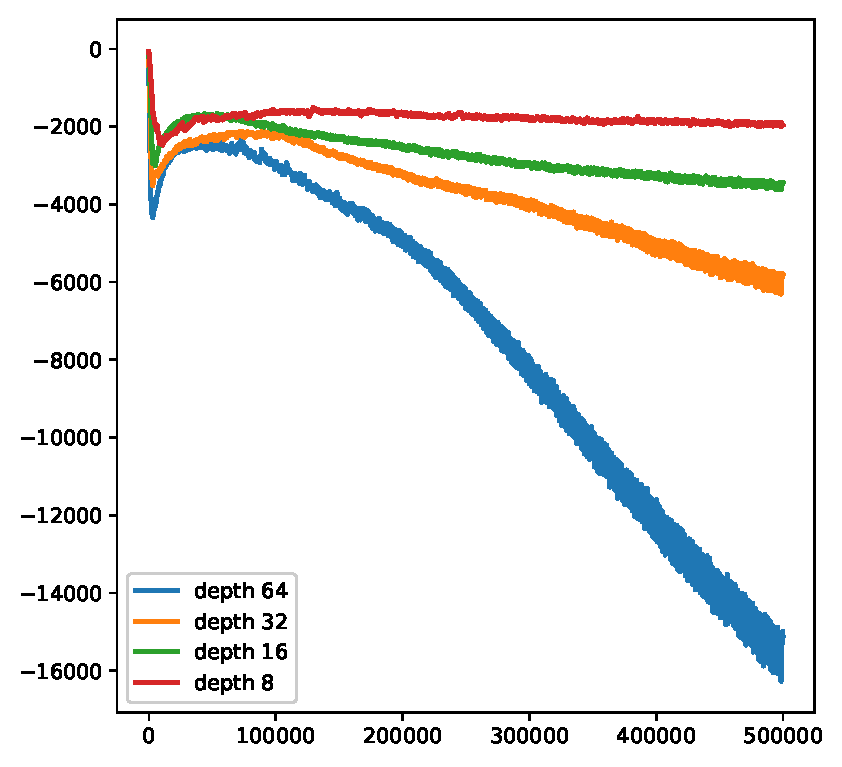
\includegraphics[width=\textwidth]{resources/images/anime_face_d_loss.eps}
        \caption{CelebA HQ}
        \label{fig:anime_face_d_loss}
    \end{subfigure}
    \caption{Discriminator loss curves}
    \label{fig:d_loss}
\end{figure}

The graphic above shows the loss curves of different models. One can see that with a higher model depth (which means more model parameters), the discriminator loss falls faster. That confirms the observations of the authors of \cite{arjovsky2017wgan}. They note that the discriminator loss correlates with the image quality. Therefore it makes sense that networks with more parameters can generate better-looking images. \\

\begin{figure}[H]
    \centering
    \begin{subfigure}[b]{0.24\textwidth}
        \centering
        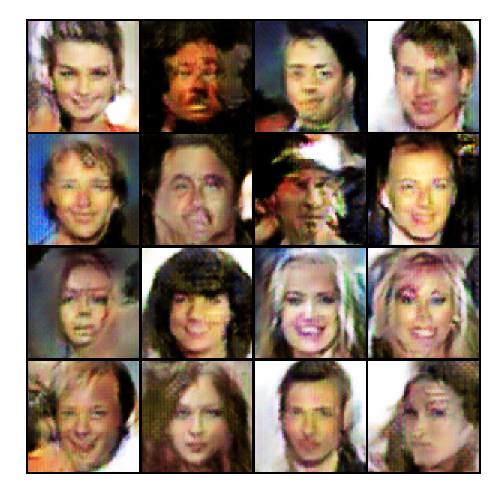
\includegraphics[width=\textwidth]{resources/images/output_celeba_8.eps}
        \caption{depth 8}
        \label{fig:celeba_8}
    \end{subfigure}
    \hfill
    \begin{subfigure}[b]{0.24\textwidth}
        \centering
        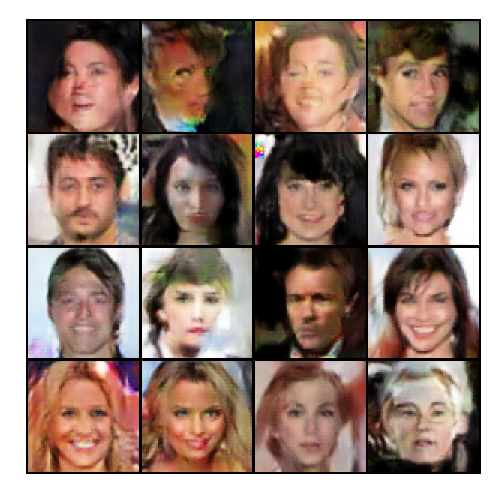
\includegraphics[width=\textwidth]{resources/images/output_celeba_16.eps}
        \caption{depth 16}
        \label{fig:celeba_16}
    \end{subfigure}
    \hfill
    \begin{subfigure}[b]{0.24\textwidth}
        \centering
        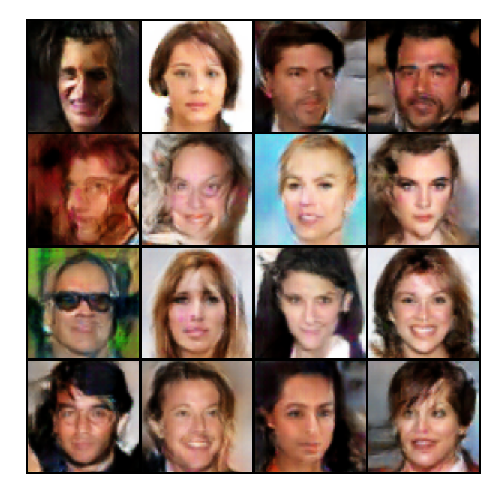
\includegraphics[width=\textwidth]{resources/images/output_celeba_32.eps}
        \caption{depth 32}
        \label{fig:celeba_32}
    \end{subfigure}
    \hfill
    \begin{subfigure}[b]{0.24\textwidth}
        \centering
        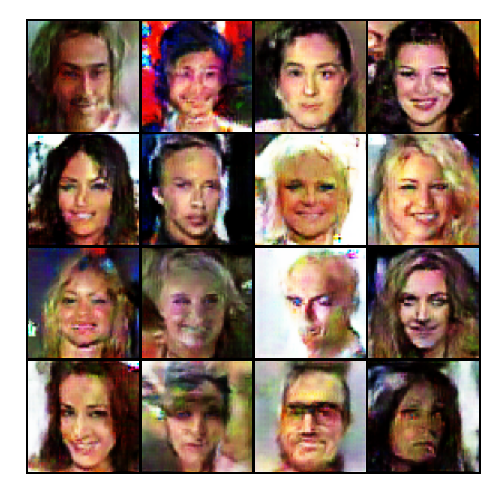
\includegraphics[width=\textwidth]{resources/images/output_celeba_64.eps}
        \caption{depth 64}
        \label{fig:celeba_64}
    \end{subfigure}
    \caption{Sample generated images of different models trained on the Celeba HQ dataset}
    \label{fig:output_celeba}
\end{figure}

The graphic above shows sample images generated by the networks trained on the Celeba QH dataset. It is clear to see that the networks with smaller depth produce less appealing photos. The images generated by the depth 8 network do clearly show many artifacts. In this experiment, the depth 32 network delivers the best results. Some of the generated pictures look almost like human faces. Others have artifacts but less than the pictures generated by the other networks. Also, this network learned about face accessories, as one person is wearing glasses on the image. The depth 64 network produces images with many artifacts. A possible reason is that the training process ran into a local minimum, which it couldn't escape from anymore. Another explanation is that a network with a depth of 64 is overparameterized, and the training process needs more time to converge.

\begin{figure}[H]
    \centering
    \begin{subfigure}[b]{0.24\textwidth}
        \centering
        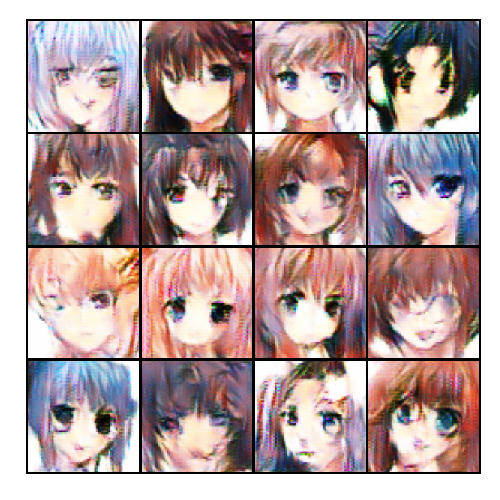
\includegraphics[width=\textwidth]{resources/images/output_anime_8.eps}
        \caption{depth 8}
        \label{fig:anime_8}
    \end{subfigure}
    \hfill
    \begin{subfigure}[b]{0.24\textwidth}
        \centering
        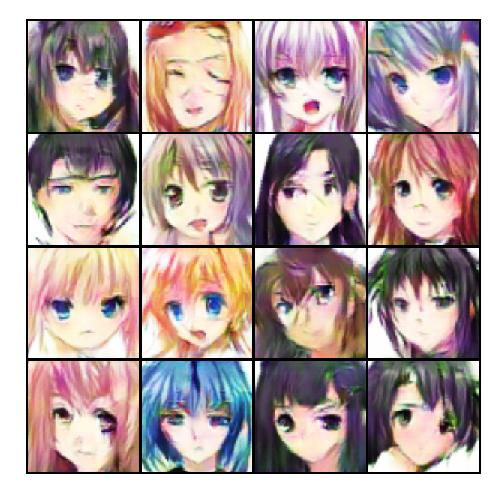
\includegraphics[width=\textwidth]{resources/images/output_anime_16.eps}
        \caption{depth 16}
        \label{fig:anime_16}
    \end{subfigure}
    \hfill
    \begin{subfigure}[b]{0.24\textwidth}
        \centering
        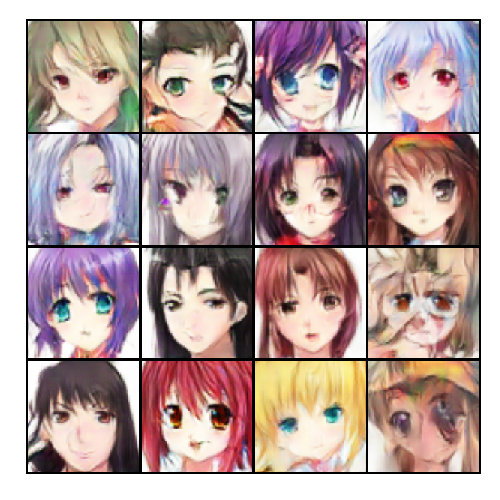
\includegraphics[width=\textwidth]{resources/images/output_anime_32.eps}
        \caption{depth 32}
        \label{fig:anime_32}
    \end{subfigure}
    \hfill
    \begin{subfigure}[b]{0.24\textwidth}
        \centering
        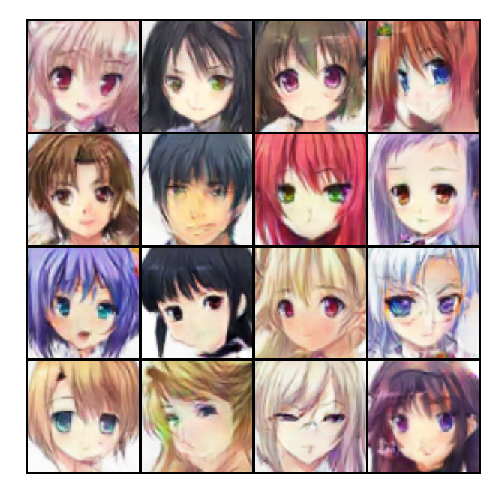
\includegraphics[width=\textwidth]{resources/images/output_anime_64.eps}
        \caption{depth 64}
        \label{fig:anime_64}
    \end{subfigure}
    \caption{Sample generated images of different models trained on the Anime Face dataset}
    \label{fig:ouput_anime}
\end{figure}

Similar observations can be made by looking at the generated pictures of the network trained on the Anime Face dataset. The networks with lower depth produce more artifacts. Also, the variety of the generated images is lower than in images generated by the higher parameterized networks. It is important to note that the depth 64 network, in this case, delivers excellent results. Most pictures look very similar to the images in the real Anime Face dataset. 

\subsection{Conclusion}

In this project, the author demonstrates how to use the GAN \cite{goodfellow2014generative} framework to generate new images of a given domain. He uses the DCGAN \cite{radford2016dcgan} architecture and the WGAN \cite{arjovsky2017wgan} loss function with gradient penalty \cite{gulrajani2017wgangp}. The experiments demonstrate the flexibility of this approach by training models on different datasets with and other numbers of parameters. The results are, as expected, not perfect because, in the chosen method, earlier technologies are used. The generation of images with a higher resolution is still more complex and requires further research. Also, networks still produce many generation artifacts, which clearly visually separates the generated images from images of the dataset.

\newpage

\subsection{Future work and improvements}

Generative Adversarial Networks are a vast research area. In future projects, it is worth improving the author's approach to image generation.   It would be meaningful to generate images of higher resolutions and with fewer image artifacts. To achieve this goal, different technologies could be used.  Other researchers use different network architectures and skip connections between generator and discriminator \cite{karnewar2020msggan}. Others use more advanced gradient penalties \cite{dragan} \cite{wgandiv}, loss functions \cite{realness} \cite{jolicoeurmartineau2018rahinge}, and normalization procedures \cite{miyato2018spectral}. It is interesting to combine certain technologies to see if they complement each other. \\

Other options are to use the gained insights to implement different types of GANs. The StyleGAN \cite{stylegan}, \cite{stylegan2} architecture has more fine-grain control over the generated images. In the image-to-image translation field, CycleGAN \cite{cyclegan} can transfer pictures of one domain to another. These fields are also fascinating research topics.
